\documentclass[runningheads]{llncs}
\usepackage[T1]{fontenc}
\usepackage{amsmath,amssymb,booktabs,graphicx,multirow}
\usepackage[hidelinks]{hyperref}
\begin{document}
\title{Hindsight Is Not Opportunity: Pre-Outcome Value in Risk-Constrained Label Acquisition with Delayed Feedback}
\titlerunning{Hindsight Is Not Opportunity}
\author{Anonymous Authors}
\authorrunning{Anonymous Authors}
\institute{Anonymous Institution}
\maketitle
\begin{abstract}
In credit and other decision systems, labels are acquired by taking risky actions, outcomes arrive with delay, and a risk budget limits which label sets are feasible. We study when the composition of a feasible set, rather than its size, determines learning value, and how much of that value a policy can realize before outcomes are known. We give a same-state quantity--composition decomposition, a closed-form threshold at which pending information reverses the preferred set under a fixed budget, and a decomposition of post-outcome headroom into a non-deployable foresight term and a pre-outcome term that we estimate directly with known outcome probabilities. A mechanism-informed reference policy, DC-PRISM, serves as the instrument. In controlled worlds, 83\% of post-outcome headroom is achievable before outcomes arrive and DC-PRISM lowers expected Brier loss by $12.2\times10^{-3}$ relative to the risk reference while acquiring about half as many labels. On real credit covariates the same headroom is 61--90\% foresight; coverage gaps enlarge the pre-outcome part, and a point-value proxy ranks it well, but the conservative layer that drives the controlled gain returns the reference set in 84--95\% of states. Online replay on four credit cohorts, with engineered and natural candidate streams and eight comparators, finds no decisive difference. The results separate hindsight from deployable opportunity and identify a conservatism trade-off in exploiting favorable information geometry.
\keywords{Selective labels \and Risk-constrained acquisition \and Delayed feedback \and Active learning \and Credit risk}
\end{abstract}

\section{Introduction}
\label{sec:intro}
A lender observes repayment only for applications it approves, so the data available for future learning depend on earlier decisions~\cite{lakkaraju2017selective,wei2021selective}. Each approval is also an exposure to loss. When outcomes arrive with delay, the learner must additionally account for decisions already taken but not yet settled. Label acquisition in such systems therefore combines a risk budget, incomplete coverage of the population, and information that is committed but still pending.

A risk budget determines which label sets are feasible, but not which feasible set is most valuable. Active learning and experimental design select observations by their expected contribution to prediction~\cite{cohn1996active,yu2006transductive,settles2009active}, and recent criteria target Fisher information, predictive information or downstream loss~\cite{ash2021fishing,bickfordsmith2023prediction,huang2026loss}. Under a risk budget, one informative but exposed observation can displace several cheap ones, so composition and quantity trade off directly. Pending outcomes change the comparison again, because information along some directions is already on its way.

This paper is a mechanism study of that trade-off. We ask three questions. (i) How do quantity and composition contribute to the realized gain of a feasible set over a quantity-oriented reference? (ii) When does pending information reverse the preferred composition under an unchanged budget? (iii) How much of the opportunity that is visible \emph{after} outcomes arrive could any policy realize \emph{before} they do? The third question matters because empirical studies of acquisition routinely compare chosen sets with the best set in hindsight. Such hindsight headroom mixes value that is achievable with the information at hand and value that requires knowing the hidden training labels.

\paragraph{Contributions.}
\begin{itemize}
\item \textbf{Mechanism analysis.} A same-state quantity--composition decomposition, and a closed-form threshold at which directional pending information makes a smaller feasible set preferable under the same budget (Sec.~\ref{sec:mechanism}).
\item \textbf{Hindsight versus pre-outcome value.} A decomposition of post-outcome headroom into foresight and pre-outcome selection terms, together with a bracketing Monte Carlo estimator that makes the terms measurable when outcome probabilities are known (Sec.~\ref{sec:opportunity}).
\item \textbf{Layered evidence.} Pre-registered experiments on controlled worlds, real credit covariates with paired coverage interventions, and delayed replay on four credit cohorts under engineered and natural candidate streams, with eight comparators. They show that the controlled opportunity is largely deployable whereas the real-covariate opportunity is mostly foresight, and they localize the remaining gap to a conservatism trade-off in the decision rule (Secs.~\ref{sec:controlled}--\ref{sec:replay}).
\end{itemize}
DC-PRISM, the policy we use as an instrument, follows from the mechanism: it compares feasible sets against the quantity reference using pending-aware, target-weighted information (Sec.~\ref{sec:policy}). We do not claim that it outperforms simple information-based baselines on real data; the experiments show where it does and does not, and why.

\section{Setting}
\label{sec:setting}
At round $t$, a learner observes labeled history $D_t$, the covariates of pending acquisitions $O_t$, an unlabeled candidate pool $C_t$ and target covariates $Q_t$. Candidate $i$ has a visible exposure $e_i\geq0$ and a binary adverse outcome $Y_i$ revealed only after acquisition and a feedback delay. A legal policy chooses $S_t\subseteq C_t$ using the visible information $\mathcal H_t$; outcomes in $O_t$ and $C_t$ stay hidden. Learning is measured with the Brier score~\cite{brier1950verification}. For a fixed state, $L(S;Y)$ denotes test loss after fitting on $D\cup O\cup S$, where $Y$ collects the hidden training outcomes of $O$ and $S$.

\paragraph{Risk-feasible sets.} Let $q_i\in[0,1]$ be a risk score available at selection, $\ell=\log(1/\alpha)$, and $\phi(q)=q(1-q)$ for $q\le1/2$, $\phi(q)=1/4$ otherwise. For nonempty $S$,
\begin{equation}
 R_\alpha(S)=\sum_{i\in S}e_iq_i+\Big(2\ell\sum_{i\in S}e_i^2\phi(q_i)\Big)^{1/2}+\frac{\ell}{3}\max_{i\in S}e_i,
 \label{eq:envelope}
\end{equation}
$R_\alpha(\varnothing)=0$, and $\mathcal A_t=\{S\subseteq C_t:R_\alpha(S)\le B_t\}$. If, conditional on $\mathcal H_t$, the selected outcomes are independent Bernoulli variables with $p_i\le q_i$, a sub-gamma bound~\cite{boucheron2013concentration} gives $\Pr\{\sum_{i\in S}e_iY_i>R_\alpha(S)\mid\mathcal H_t\}\le\alpha$. Our experiments use empirical Wilson/Laplace scores, for which these conditions are not guaranteed; we use~\eqref{eq:envelope} as the operational feasible region shared by all policies.

\paragraph{Quantity reference.} The reference $M_K\in\mathcal A_t$ maximizes cardinality and breaks ties by smaller envelope; $K=|M_K|$. Small pools are enumerated; larger pools use exposure-stratified search with a cardinality upper bound.

\section{Mechanism Analysis}
\label{sec:mechanism}
\subsection{Quantity and Composition}
For a selected $S$ with $|S|=k\le K$, let $M_k$ be a feasible risk-ranked reference of size $k$ (with $M_K$ reused when $k=K$). From the same $D\cup O$ and realized outcomes,
\begin{equation}
\begin{gathered}
 Q_k=L(M_k;Y)-L(M_K;Y),\qquad C_k=L(M_k;Y)-L(S;Y),\\
 J=L(M_K;Y)-L(S;Y)=C_k-Q_k.
\end{gathered}
 \label{eq:decomposition}
\end{equation}
$Q_k$ compares two risk references of different size; $C_k$ compares equally sized sets. $J>0$ means composition more than compensates for the quantity term. $Q_k$ need not be positive: a larger reference can have higher test loss.

\subsection{Directional Pending Information}
Consider a two-parameter linear Gaussian model with precision $H=\operatorname{diag}(h_1,h_2)$, target weights $G=\operatorname{diag}(g_1,g_2)$, and loss $\operatorname{tr}(GH^{-1})$. Pending observations add precision $o\ge0$ along direction~1. The quantity reference adds precision $a$ along direction~1; a smaller alternative adds $b$ along direction~2. Both remain feasible as $o$ varies.

\begin{proposition}[Directional preference reversal]
The gain of the alternative over the reference is
$J(o)=\frac{g_2b}{h_2(h_2+b)}-\frac{g_1a}{(h_1+o)(h_1+o+a)}$, which is strictly increasing in $o$. With $v_2=g_2b/[h_2(h_2+b)]$, the alternative is preferred exactly when
\begin{equation}
 o>o^*=\tfrac12\big(-a+\sqrt{a^2+4g_1a/v_2}\big)-h_1 .\label{eq:threshold}
\end{equation}
\end{proposition}
\begin{proof}
The losses are $g_1/(h_1+o+a)+g_2/h_2$ and $g_1/(h_1+o)+g_2/(h_2+b)$; subtracting gives $J(o)$, whose derivative $g_1a[2(h_1+o)+a]/[(h_1+o)^2(h_1+o+a)^2]$ is positive. Solving $(h_1+o)(h_1+o+a)>g_1a/v_2$ gives~\eqref{eq:threshold}.
\end{proof}
The reversal occurs under a fixed exposure budget. With $h_j=g_j=1$, four unit-information labels on direction~1 ($a=4$) against one on direction~2 ($b=1$), $\alpha=0.1$ and $q=0.1$, exposures $0.1$ per reference label and $0.1624$ for the alternative give both actions envelope $B\approx0.2455$, and no mixture is feasible. The reference is preferred at $o=0$ (loss $1.20$ versus $1.50$), the alternative at $o=1$ ($1.17$ versus $1.00$), and $o^*\approx0.464$ (Fig.~\ref{fig:reversal}). Pending information lowers the value of another observation on the reference axis and leaves the other axis unchanged; candidates must therefore be valued against history \emph{plus} pending information.

\begin{figure}[t]
 \centering
 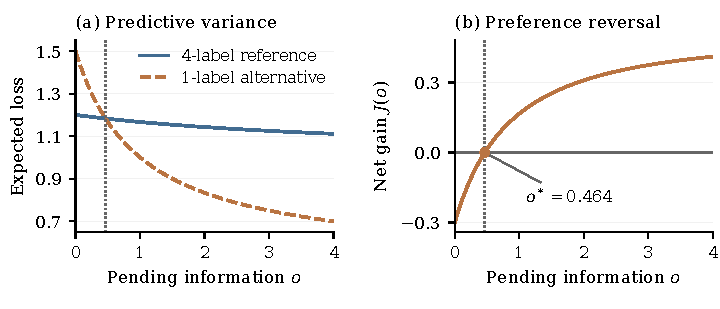
\includegraphics[width=0.92\linewidth]{figures/fig_information_reversal.pdf}
 \caption{Preference reversal in the two-direction model under a fixed risk budget. The one-label alternative becomes preferable at $o^*\approx0.464$.}
 \label{fig:reversal}
\end{figure}

\subsection{Hindsight Versus Pre-Outcome Opportunity}
\label{sec:opportunity}
Fix $\mathcal H$ and a finite family $\mathcal F$ of sets constructed from visible information and containing $M=M_K$. Let $L(S,Y)$ integrate test-label noise but keep the hidden training labels $Y$. Define
\begin{align}
 H_{\mathrm{post}}&=\mathbb E\big[L(M,Y)-\min_{S\in\mathcal F}L(S,Y)\mid\mathcal H\big],\\
 H_{\mathrm{pre}}&=\mathbb E[L(M,Y)\mid\mathcal H]-\min_{S\in\mathcal F}\mathbb E[L(S,Y)\mid\mathcal H].
\end{align}
Since the expectation of a minimum is at most the minimum of expectations, $H_{\mathrm{post}}\ge H_{\mathrm{pre}}\ge0$. For any legal policy $\pi$ choosing within $\mathcal F$ with expected gain $G_\pi=\mathbb E[L(M,Y)-L(\pi,Y)\mid\mathcal H]$,
\begin{equation}
 H_{\mathrm{post}}-G_\pi=\underbrace{H_{\mathrm{post}}-H_{\mathrm{pre}}}_{\text{foresight}}+\underbrace{H_{\mathrm{pre}}-G_\pi}_{\text{pre-outcome selection gap}} .\label{eq:opportunity}
\end{equation}
Foresight is unavailable to any deployable policy; only the second term can be closed by better selection. Hindsight comparisons with the realized best set estimate $H_{\mathrm{post}}$ and therefore overstate deployable opportunity.

\paragraph{Estimation.} When the outcome probabilities $p$ are known, we draw $R$ replicates $Y^{(r)}$ of the hidden training labels and evaluate every $S\in\mathcal F$ on all replicates with common draws. $H_{\mathrm{post}}$ is estimated without bias. The plug-in $\widehat H_{\mathrm{pre}}$, which minimizes the replicate mean, is biased upward because it selects on noise. A two-fold cross-fitted estimate, which chooses $S^\star$ on even replicates and evaluates it on odd ones (and vice versa), is biased downward. Together they bracket $H_{\mathrm{pre}}$, and $H_{\mathrm{post}}-\widehat H_{\mathrm{pre}}^{\text{plug-in}}$ is a conservative estimate of foresight.

\section{DC-PRISM: A Mechanism-Informed Reference Policy}
\label{sec:policy}
DC-PRISM values a feasible set by the target-weighted Brier reduction it would add to history and pending information, and compares it with the quantity reference. With an $\ell_2$-regularized logistic model, $\bar x=(1,x^\top)^\top$, $p_\theta(x)=\sigma(\bar x^\top\theta)$ and $w_\theta=p_\theta(1-p_\theta)$, let
\begin{gather*}
 H_{D+O}(\theta)=\Lambda+\!\!\sum_{i\in D\cup O}\!\!w_\theta(x_i)\bar x_i\bar x_i^\top,\qquad
 A_S(\theta)=\sum_{i\in S}w_\theta(x_i)\bar x_i\bar x_i^\top,\\
 G_Q(\theta)=\tfrac1{|Q|}\sum_{j\in Q}w_\theta(x_j)^2\bar x_j\bar x_j^\top,
\end{gather*}
\begin{equation}
 V_\theta(S)=\operatorname{tr}\!\big[G_Q(\theta)\{H_{D+O}(\theta)^{-1}-(H_{D+O}(\theta)+A_S(\theta))^{-1}\}\big].\label{eq:value}
\end{equation}
$V_\theta$ is a local quadratic proxy for target Brier reduction in the spirit of transductive design and predictive-information acquisition~\cite{yu2006transductive,bickfordsmith2023prediction}; pending covariates enter $H_{D+O}$ without their labels, which is exactly the discounting of an already-covered direction in the proposition.

\paragraph{Decision rule.} The candidate family contains $M_K$, value-per-envelope-cost prefixes, value-ranked prefixes and exchanges that keep part of $M_K$, all checked against~\eqref{eq:envelope}. For $m=1,\dots,M$ draws $\theta^{(m)}\sim\mathcal N(\widehat\theta,H_D^{-1})$~\cite{mackay1992practical}, candidate curvature is damped by $\exp[-0.45\{\bar x_i^\top(\theta^{(m)}-\widehat\theta)\}^2]$, and with $a_m=\max\{V_m(M_K),10^{-6}\}$,
\begin{equation}
 Z(S)=\operatorname{quantile}_{0.2}\Big\{\tanh\frac{V_m(S)-a_m}{2.5a_m}\Big\}_m-0.22\,\frac{(K-|S|)_+}{\max(K,1)} .\label{eq:score}
\end{equation}
DC-PRISM chooses $\arg\max Z$ if $Z>0.08$ and $M_K$ otherwise. The lower quantile, curvature damping and reference normalization make the rule \emph{conservative}: a smaller set must improve on $M_K$ under most parameter draws. Risk scores $q$ come from a one-sided Wilson adjustment~\cite{wilson1927probable} of the upper half of fitted historical risks combined with a high quantile over 40 Laplace logit draws. All constants were fixed before the experiments reported here; Sec.~\ref{sec:controlled} reports their sensitivity.

\paragraph{Comparators.} All policies share the state, $q$, the numerical budget and~\eqref{eq:envelope}. \emph{Safe-MinRisk} returns $M_K$. \emph{Fixed count} selects $\lceil0.75K\rceil$ labels by point value. \emph{Fisher-cost} greedily packs by single-observation parameter-variance reduction per exposure cost. Four further baselines pack greedily until no feasible candidate remains: \emph{Random}; \emph{Uncertainty}, ordered by $\widehat p(1-\widehat p)$~\cite{lewis1994sequential}; \emph{BAIT-greedy}, forward greedy on $\operatorname{tr}(F_Q(H_{D+O}+A_S)^{-1})$ with the pool Fisher matrix $F_Q$~\cite{ash2021fishing}; and \emph{TargetVar-greedy}, forward greedy on~\eqref{eq:value}, an EPIG-style Laplace approximation~\cite{bickfordsmith2023prediction} that uses DC-PRISM's proxy without its reference comparison, quantile, penalty or gate.

\section{Controlled Evidence}
\label{sec:controlled}
\paragraph{Design.} Each world has six features, 80 historical labels with narrow coverage, 22 pending acquisitions concentrated on one direction, 24 candidates, 180 target and 240 test points. Candidate groups contain low-risk core observations, pending-aligned observations, observations on two further predictive directions, and auxiliary-tail observations whose outcomes follow a piecewise regime that a logistic model cannot represent. All selections are locked before any hidden label is read. Every study below fixed its world counts, seeds, comparison families and a material-effect threshold of $5\times10^{-4}$ Brier before running. We report paired means with 95\% Bonferroni simultaneous $t$ intervals and Holm-adjusted tests~\cite{holm1979simple} within each family.

\paragraph{Realized gains and their composition.} In 128 archived worlds DC-PRISM attains Brier $0.1202$ with $3.27$ labels, against $0.1367$ for Safe-MinRisk with six labels and $0.1367$ for a four-label fixed-count rule (paired excess $16.5\times10^{-3}$, 95\% CI $[11.0,22.0]\times10^{-3}$). The same-state decomposition gives $C_k=16.3$, $Q_k=-0.19$ and $J=16.4$ ($\times10^{-3}$): the gain comes from composition, and the smaller risk reference is no worse than the larger one.

\paragraph{Fresh worlds, ex-ante endpoint.} In 128 fresh worlds we score every policy by expected Brier, integrating test-label noise exactly and training-label noise over 128 replicates (Table~\ref{tab:controlled}). DC-PRISM has the lowest loss. Its gains over Safe-MinRisk ($12.2$, simultaneous interval $[7.6,16.8]$), Fisher-cost ($17.8$, $[13.2,22.4]$), Random ($9.7$, $[5.1,14.4]$) and fixed count ($9.6$, $[5.1,14.2]$) are material. Its gains over Uncertainty, BAIT-greedy and TargetVar-greedy are $2.7$--$4.2$, but those intervals include zero (all $\times10^{-3}$).

\begin{table}[t]
\caption{Fresh controlled worlds (128): ex-ante expected Brier, mean labels, and DC-PRISM's gain with 95\% simultaneous intervals ($\times10^{-3}$; positive favors DC-PRISM).}
\label{tab:controlled}
\centering\small
\begin{tabular}{lrrr}
\toprule
Policy & Expected Brier & Labels & Gain of DC-PRISM \\
\midrule
Safe-MinRisk & 0.1384 & 6.00 & $12.2$ [$7.6$, $16.8$] \\
Fixed count & 0.1358 & 5.00 & $9.6$ [$5.1$, $14.2$] \\
Random & 0.1359 & 3.54 & $9.7$ [$5.1$, $14.4$] \\
Uncertainty & 0.1304 & 2.81 & $4.2$ [$-0.8$, $9.2$] \\
Fisher-cost & 0.1440 & 2.67 & $17.8$ [$13.2$, $22.4$] \\
BAIT-greedy & 0.1289 & 2.22 & $2.7$ [$-1.3$, $6.7$] \\
TargetVar-greedy & 0.1290 & 2.19 & $2.8$ [$-1.2$, $6.9$] \\
DC-PRISM & \textbf{0.1262} & 3.12 & -- \\
\bottomrule
\end{tabular}
\end{table}

\paragraph{Opportunity.} Here $H_{\mathrm{post}}=22.2\times10^{-3}$ and $H_{\mathrm{pre}}\in[18.4,18.5]\times10^{-3}$: 83\% of hindsight headroom is achievable before outcomes arrive, and DC-PRISM captures two thirds of it (Fig.~\ref{fig:opportunity}, left). DC-PRISM departs from $M_K$ in 96\% of worlds.

\paragraph{Components and constants.} In a common-family study that varies one component at a time, gains from the lower quantile and pending rescoring have positive means, $3.9$ and $3.0\times10^{-3}$, but intervals that include zero; the gate and quantity penalty have means within $\pm0.3\times10^{-3}$. Changing any single constant (quantile $0.1$--$0.5$, penalty $0$--$0.44$, gate $0$--$0.16$, damping $0$--$0.9$, tanh scale $1.25$--$5$) changes expected loss by at most $1.3\times10^{-3}$; in these worlds the gate never changes expected loss by more than $3\times10^{-5}$. The controlled gain is therefore a property of the conservative, pending-aware comparison as a whole rather than of a tuned constant or an isolated component.

\section{Real Covariates: Where the Opportunity Goes}
\label{sec:realx}
\paragraph{Design.} We keep the real covariates of HMEQ and LendingClub and generate outcomes from a known logistic or nonlinear logit ($p(x)=\sigma(-0.8+x^\top\beta)$, optionally plus $0.5\sin x_2+0.35x_3x_4$), so that $H_{\mathrm{pre}}$ is measurable. In each of 64 fresh pairs per setting, a 240-record reservoir supplies two histories: \emph{broad} (80 random records) and \emph{gap} (the 80 lowest on the second feature). Candidates, pending and target records, labels, preprocessing, risk scores, budget, reference and family are identical across arms, so the pair isolates history coverage.

\paragraph{Most hindsight headroom is foresight.} Table~\ref{tab:realx} and Fig.~\ref{fig:opportunity} show that $H_{\mathrm{post}}$ is an order of magnitude smaller than in the controlled worlds and, more importantly, mostly foresight: the pre-outcome share is 10--39\% across the eight arms (foresight 61--90\%), against 83\% in controlled worlds. Coverage gaps more than double $H_{\mathrm{post}}$ (from $1.9$--$2.4$ to $4.9$--$6.4\times10^{-3}$) and raise $H_{\mathrm{pre}}$ to at most $1.9\times10^{-3}$. Foresight is materially positive in all nine groups. An earlier independent batch of 256 pairs showed a similar increase in post-outcome headroom (material in three of four settings).

\begin{table}[t]
\caption{Real-covariate states (64 pairs per setting; $\times10^{-3}$ expected Brier). $H_{\mathrm{pre}}$ is bracketed by the cross-fitted and plug-in estimates. ``Proxy'' chooses $\arg\max_{\mathcal F}V_{\widehat\theta}$; $\rho$ is the Spearman correlation between $V_{\widehat\theta}$ and the true ex-ante gain across $\mathcal F$; ``$=M_K$'' is the share of states where DC-PRISM returns the reference.}
\label{tab:realx}
\centering\small
\setlength{\tabcolsep}{2.5pt}
\begin{tabular}{llrrrrrr}
\toprule
Setting & Arm & $H_{\mathrm{post}}$ & $H_{\mathrm{pre}}$ & DC gain & Proxy gain & $=M_K$ & $\rho$ \\
\midrule
HMEQ, logistic & broad & 2.19 & [0.48, 0.58] & 0.04 & 0.12 & 86\% & 0.27 \\
 & gap & 6.37 & [1.49, 1.87] & $-0.04$ & 0.81 & 88\% & 0.64 \\
HMEQ, nonlinear & broad & 2.43 & [0.85, 0.94] & $-0.02$ & 0.09 & 84\% & 0.31 \\
 & gap & 5.83 & [1.51, 1.89] & 0.10 & 0.66 & 95\% & 0.55 \\
LC, logistic & broad & 2.00 & [0.29, 0.39] & 0.04 & 0.03 & 92\% & 0.33 \\
 & gap & 4.88 & [0.51, 0.83] & 0.02 & 0.24 & 92\% & 0.69 \\
LC, nonlinear & broad & 1.89 & [0.31, 0.41] & 0.01 & 0.02 & 88\% & 0.14 \\
 & gap & 5.16 & [0.64, 0.96] & 0.04 & 0.26 & 95\% & 0.65 \\
\midrule
Controlled & -- & 22.21 & [18.38, 18.53] & 12.19 & 4.94 & 4\% & $-0.01$ \\
\bottomrule
\end{tabular}
\end{table}

\begin{figure}[t]
 \centering
 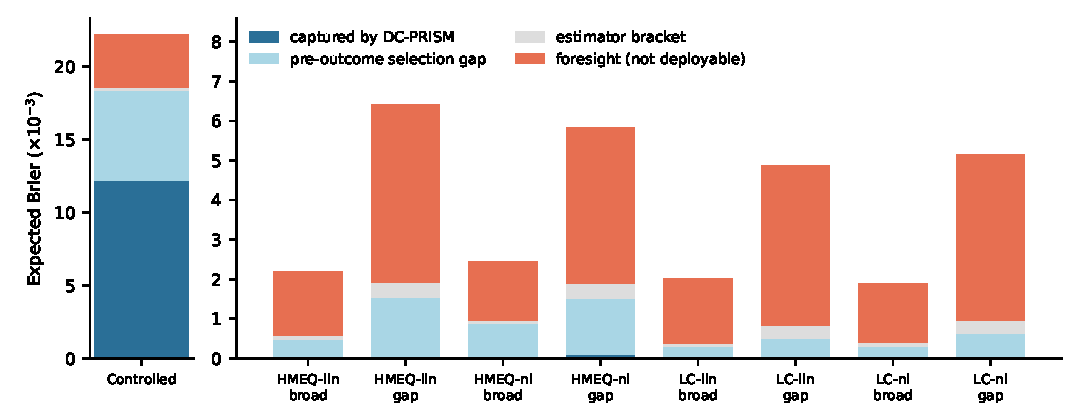
\includegraphics[width=\linewidth]{figures/supplement_v3_opportunity.pdf}
 \caption{Decomposition of post-outcome headroom~\eqref{eq:opportunity}. Gray: gap between plug-in and cross-fitted estimates of $H_{\mathrm{pre}}$. Left: controlled worlds; right: real-covariate arms (lin/nl outcome model, broad/gap history). Note the different scales.}
 \label{fig:opportunity}
\end{figure}

\paragraph{Locating the pre-outcome gap.} DC-PRISM's ex-ante gain is within $\pm0.1\times10^{-3}$ in every arm, so its selection gap equals almost all of $H_{\mathrm{pre}}$. To locate it, we rank the same family by $V_\theta$ at the fitted parameter $\widehat\theta$ and at the population parameter $\theta_{\mathrm{pop}}$ (the KL projection of the true $p$ onto the logistic class, equal to the true parameter in logistic settings). On real covariates, neither the parameter effect (gain at $\theta_{\mathrm{pop}}$ minus gain at $\widehat\theta$, means $0.02$--$0.61$) nor the remaining approximation gap ($H_{\mathrm{pre}}$ minus gain at $\theta_{\mathrm{pop}}$, means $0.09$--$0.40$) is material in any of the 16 registered tests ($\times10^{-3}$). Under coverage gaps the proxy ranks the family well ($\rho=0.55$--$0.69$), and choosing its maximizer captures 41--54\% of the cross-fitted $H_{\mathrm{pre}}$ in all four gap settings (Table~\ref{tab:realx}). In the controlled worlds the picture is reversed: the proxy's ranking is uninformative ($\rho\approx0$), ranking at $\theta_{\mathrm{pop}}$ is materially \emph{worse} than at $\widehat\theta$ ($-11.2$, interval $[-15.7,-6.6]$), and the approximation gap is material ($18.9$, $[14.2,23.5]$), consistent with the auxiliary-tail regime that the logistic class misspecifies.

\paragraph{A conservatism trade-off.} Together these results suggest the following mechanism; we label it exploratory because it combines registered endpoints with descriptive comparisons. Where the local proxy is unreliable, as in the misspecified controlled tails, DC-PRISM's reference-relative, lower-quantile, damped comparison turns an uninformative ranking into a large gain ($12.2$ against $4.9$ for the proxy maximizer). Where the proxy is reliable, as on real covariates with coverage gaps, the same conservatism keeps the reference set in 84--95\% of states and forgoes the part of $H_{\mathrm{pre}}$ that the proxy alone would capture. Consistent with this, the gate and quantity penalty barely matter on real covariates, and the largest single-constant changes there come from damping and quantile, though all remain below $0.25\times10^{-3}$. The absolute amounts at stake on real covariates are small: at most $1.9\times10^{-3}$ Brier is deployable in our settings.

\section{Delayed Replay on Real Labels}
\label{sec:replay}
\paragraph{Protocol.} We replay ten rounds on processed HMEQ, LendingClub, PPDai and UCI Credit cohorts with six features and recorded binary outcomes~\cite{sasHMEQ,lendingclubSource,ppdaiSource,yeh2009comparison}. Each seed reserves 1{,}000 test rows, 600 target rows and a 600-row history window from which 68 initial records are taken. Each round offers 24 candidates and 14 ordinary acquisitions. Exploration labels arrive one round after selection and ordinary labels two rounds after, and Brier loss is measured at the start of each round, after due releases. ALC-Brier averages the ten round scores. Preprocessing is fitted on the initial history, and the numerical budget is fixed across policies from the initial model. We use two streams. The \emph{engineered} stream ranks observable covariates to supply low-risk, pending-aligned, complementary and tail candidates from a narrow initial history, mirroring the controlled design. The \emph{natural} stream draws the initial history and every round's records at random. Each stream uses 32 fresh split seeds per cohort and nine policies; DC-PRISM is compared with each of seven comparators in a 56-test family.

\begin{table}[t]
\caption{Delayed replay: mean ALC-Brier ($\times10^{-2}$) over 32 seeds per cohort. Seed-level standard deviations are 0.7--3.1 in these units, an order of magnitude above most policy differences.}
\label{tab:replay}
\centering\small
\setlength{\tabcolsep}{3.5pt}
\begin{tabular}{lrrrrrrrr}
\toprule
& \multicolumn{4}{c}{Engineered stream} & \multicolumn{4}{c}{Natural stream} \\
\cmidrule(lr){2-5}\cmidrule(lr){6-9}
Policy & HMEQ & LC & PPDai & UCI & HMEQ & LC & PPDai & UCI \\
\midrule
Ordinary only & 16.87 & 17.05 & 12.83 & 17.85 & 13.84 & 15.72 & 11.72 & 15.98 \\
Safe-MinRisk & 16.95 & 16.81 & 12.64 & 17.76 & 13.73 & 15.59 & 11.61 & 15.85 \\
Fixed count & 16.96 & 16.85 & 12.49 & 17.76 & 13.70 & 15.61 & 11.58 & 15.85 \\
Random & 16.81 & 16.85 & 12.58 & 17.80 & 13.73 & 15.67 & 11.62 & 15.87 \\
Uncertainty & 16.79 & 16.97 & 12.39 & 17.77 & 13.73 & 15.63 & 11.53 & 15.79 \\
Fisher-cost & 16.65 & 16.55 & 12.48 & 17.80 & 13.62 & 15.60 & 11.61 & 15.86 \\
BAIT-greedy & 16.67 & 16.54 & 12.50 & 17.83 & 13.56 & 15.62 & 11.52 & 15.82 \\
TargetVar-greedy & 16.65 & 16.57 & 12.51 & 17.82 & 13.60 & 15.60 & 11.53 & 15.82 \\
DC-PRISM & 16.66 & 16.65 & 12.35 & 17.75 & 13.67 & 15.56 & 11.55 & 15.85 \\
\bottomrule
\end{tabular}
\end{table}

\begin{figure}[t]
 \centering
 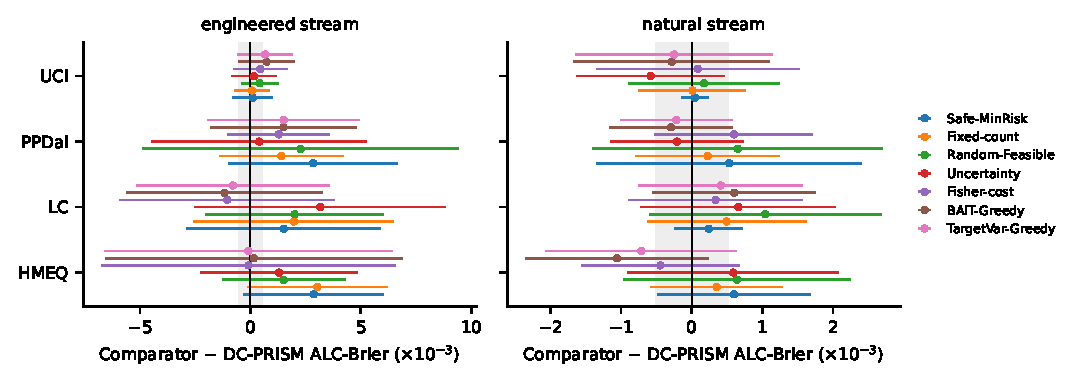
\includegraphics[width=\linewidth]{figures/supplement_v3_online.pdf}
 \caption{Comparator minus DC-PRISM ALC-Brier with 95\% simultaneous intervals over the 56-test family; positive favors DC-PRISM. Gray band: $\pm5\times10^{-4}$.}
 \label{fig:replay}
\end{figure}

\paragraph{Results.} No comparison in the 56-test family is decisive (Fig.~\ref{fig:replay}). On the engineered stream, DC-PRISM's mean is lower than that of the quantity-oriented policies (Safe-MinRisk, fixed count, Random) by $1.4$--$3.0\times10^{-3}$ on HMEQ, LendingClub and PPDai, and is within $\pm1.5\times10^{-3}$ of the information-based policies (Fisher-cost, BAIT-greedy, TargetVar-greedy). On the natural stream, all policies are within $1.1\times10^{-3}$ of DC-PRISM; on UCI Credit its difference from Safe-MinRisk lies inside the material band. An earlier 16-seed batch had found one material gain, over fixed count on PPDai ($4.1\times10^{-3}$); this larger study does not reproduce it ($1.4$, interval $[-1.4,4.2]\times10^{-3}$). DC-PRISM acquires $3.9$--$6.5$ labels per round, against $2.4$--$4.6$ for BAIT- and TargetVar-greedy. All envelope-constrained policies stay within their budgets in every round. The replay agrees with Sec.~\ref{sec:realx}: on real outcomes the opportunity that remains after foresight is small, and the policies that exploit it are statistically indistinguishable at this sample size.

\section{Related Work}
\label{sec:related}
\paragraph{Prediction-oriented and batch acquisition.} Active learning selects observations to improve a predictive model~\cite{cohn1996active,settles2009active}, from uncertainty sampling~\cite{lewis1994sequential} to criteria based on transductive design~\cite{yu2006transductive}, Fisher embeddings (BAIT)~\cite{ash2021fishing}, gradient diversity~\cite{ash2020badge}, joint mutual information~\cite{kirsch2019batchbald}, predictive information (EPIG)~\cite{bickfordsmith2023prediction} and decision loss~\cite{huang2026loss}. Cost-sensitive and budgeted variants allocate heterogeneous annotation cost~\cite{tomanek2010cost,morato2025conbatch}. These methods supply the information geometry we use. We study a different object: how an exposure-based feasible region and pending information change the relative value of quantity and composition, and how much of the resulting opportunity is deployable.

\paragraph{Selective labels, safety and delay.} Selective-label work formalizes outcomes revealed only by favorable decisions~\cite{lakkaraju2017selective}; Wei~\cite{wei2021selective}, Kilbertus et al.~\cite{kilbertus2020fair} and Keswani et al.~\cite{keswani2024partial} study policies that trade exploration against utility, fairness or coverage, and logged data can seed further experimentation~\cite{yan2018logged}. In credit scoring, reject inference attempts to correct for the missing outcomes of rejected applicants~\cite{crook2004reject}. Safe exploration~\cite{sui2015safe} and conservative bandits~\cite{wu2016conservative} constrain exploration by a safety or baseline-performance requirement, and online learning with delayed feedback~\cite{joulani2013delayed,chapelle2014delayed} and latency-aware active learning~\cite{pham2022latency} account for outcomes that arrive late. Our setting combines these elements but asks a mechanism question that they do not isolate: holding the state and risk budget fixed, which feasible composition is worth more, and how much of the apparent advantage could be known before outcomes arrive.

\section{Discussion and Conclusion}
\label{sec:conclusion}
Hindsight comparisons with the best realized set are a natural way to show that a selection rule ``leaves value on the table''. Our decomposition shows they can mislead. In controlled worlds built around directional pending information and misspecified tails, most hindsight headroom is deployable, and a conservative pending-aware comparison captures much of it with fewer labels. On real credit covariates, most of the same headroom is foresight. What remains grows with coverage gaps and is well ranked by a local information proxy, but a conservative decision rule leaves it unused. In online replay, information-based policies, including DC-PRISM, cannot be separated from one another.

\paragraph{Limitations.} Real-covariate outcomes are generated from known probabilities, because measuring $H_{\mathrm{pre}}$ requires them. Replay uses fixed processed cohorts with random rather than calendar splits, and we do not claim external or temporal validation. The risk envelope's probability guarantee requires simultaneous coverage by $q$, which our empirical scores do not ensure. BAIT-greedy (forward step only) and TargetVar-greedy (a Laplace approximation to EPIG) are adaptations, not full reimplementations. The conservatism trade-off is an exploratory synthesis of registered endpoints.

\paragraph{Outlook.} The results point to two concrete directions: diagnosing proxy reliability from visible information, so that conservatism can be relaxed where the proxy ranks well; and reporting pre-outcome rather than hindsight headroom when acquisition rules are evaluated. Code, frozen protocols, aggregate results and verifiers are available in an anonymized repository.

\bibliographystyle{splncs04}
\bibliography{refs}
\end{document}
